\chapter{Data Analysis}\label{chap:02}

Before starting our analysis of the real LHCb data, it is good practice to test and improve our analysis strategy on simulated data. This preliminary procedure is actually a common practice. In a simulation, we work under the assumption of a perfect detector with no background (only signal events) while the analysis of real events is more challenging.

\section{Real and simulated data}

\begin{figure}[H]
    \centering
    \subfloat[LHCb data of reconstructed invariant mass.]{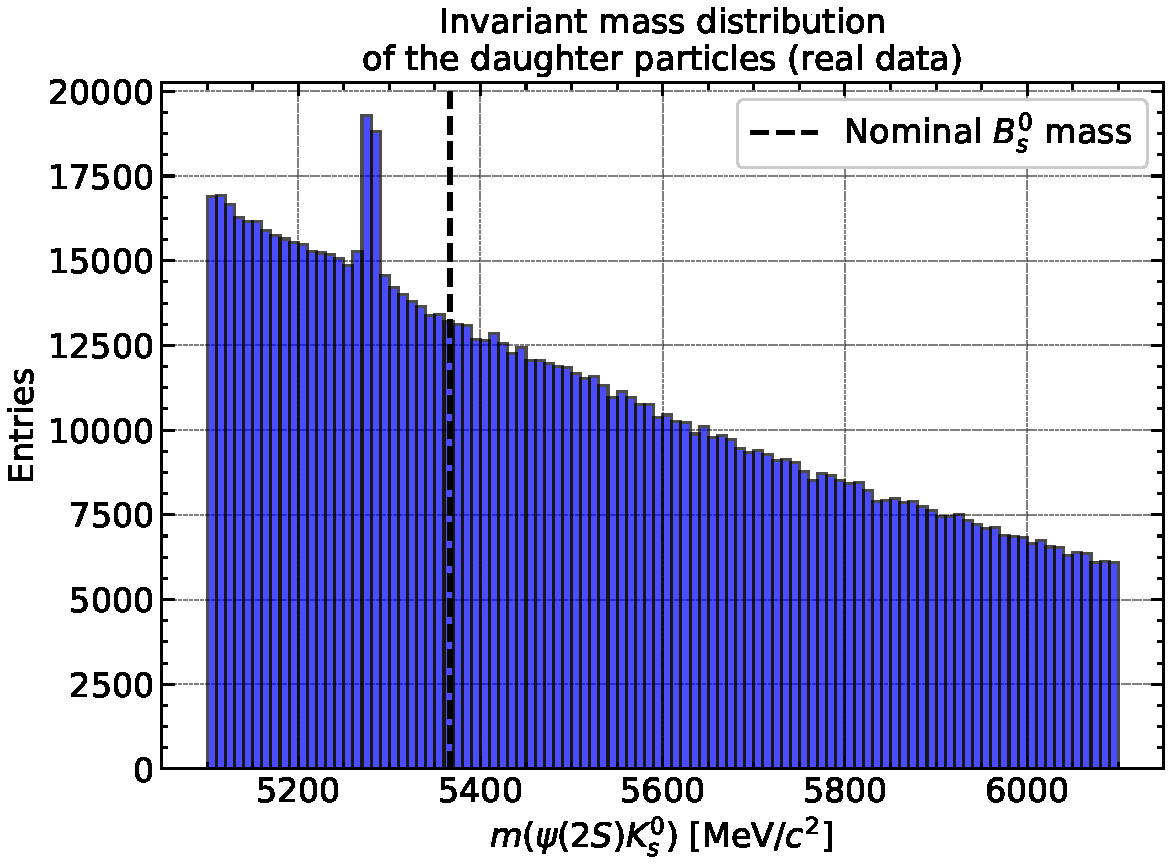
\includegraphics[width=0.3\linewidth]{graphs/m_B0_real.pdf}\label{predatasets1}}
    \hfill % \hskip 1ex
    \subfloat[Signal simulation for $B_{s}^{0}$ decay.]{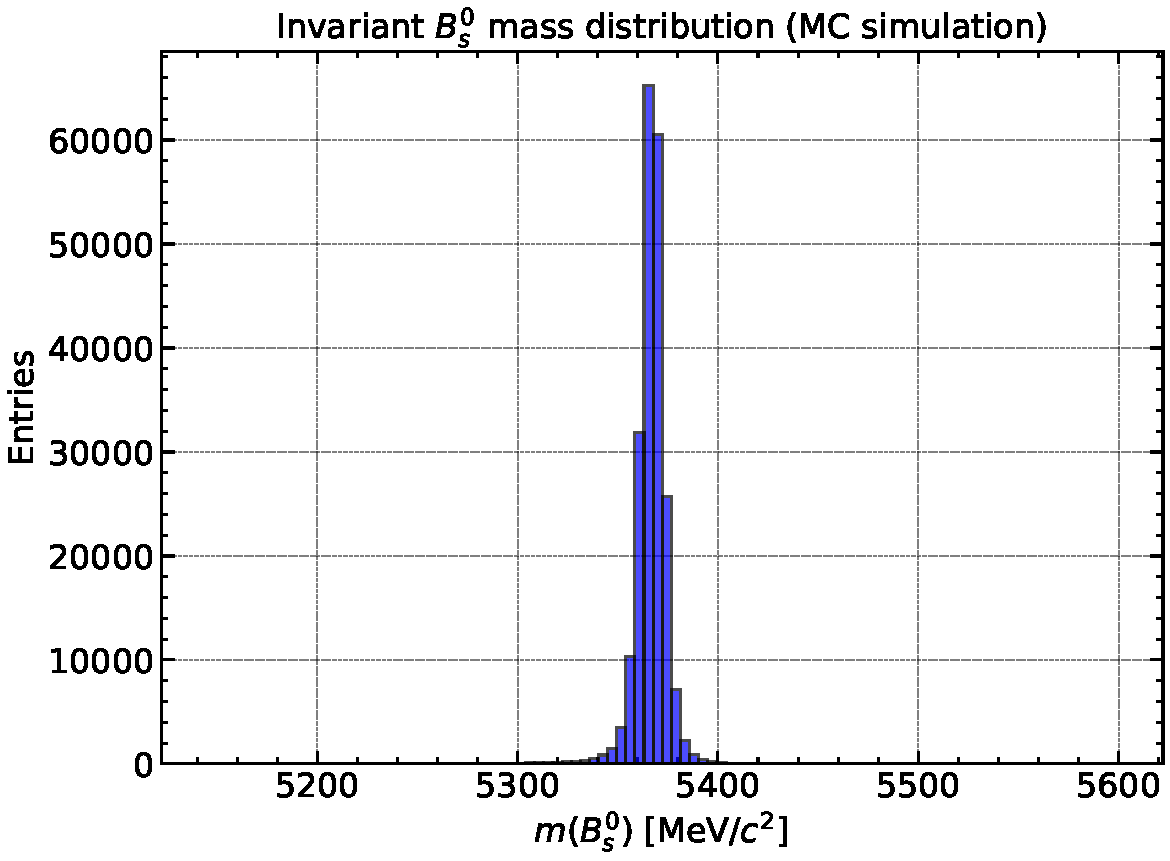
\includegraphics[width=0.3\linewidth]{graphs/m_B0S_MC.pdf}\label{predatasets2}}
    \hfill
    \subfloat[Signal simulation for $B_{d}^{0}$ decay.]{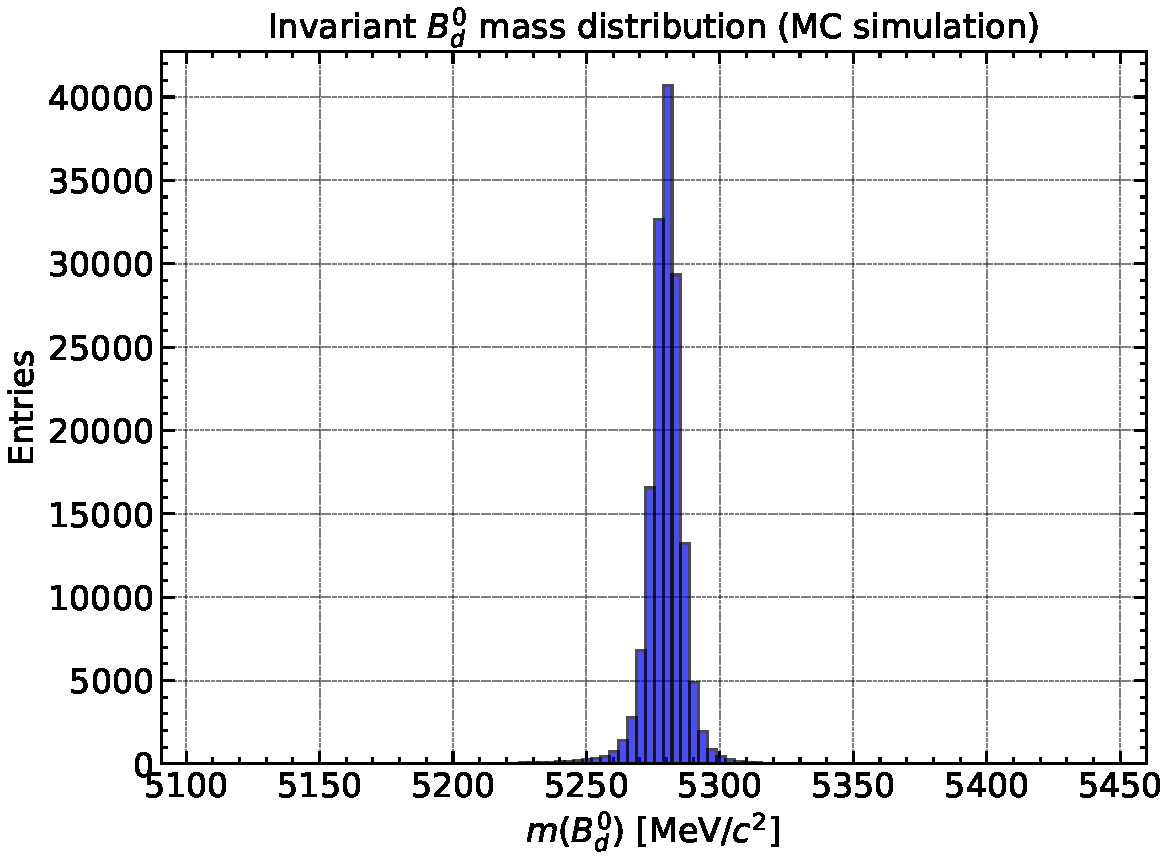
\includegraphics[width=0.3\linewidth]{graphs/m_B0D_MC.pdf}\label{predatasets3}}
    \caption{}
    \label{predatasets}
\end{figure}

For the analysis of $B_{s}^{0}\rightarrow \psi(2S)K_{S}$, we are going to use three data samples:

\begin{itemize}
    \item Real data collected from the LHCb;
    \item Monte-Carlo simulation of the signal decay $B_{s}^{0}\rightarrow \psi(2S)K_{S}^{0}$;
    \item Monte-Carlo simulation of the signal decay $B_{d}^{0}\rightarrow \psi(2S)K_{S}^{0}$, (kinematically similar decay).
\end{itemize}
Of which the LHCb data has already went through heavy pre-selection via trigger, track reconstruction, etc.\ while the distributions and the peaks of $B_{s}^{0}$ and $B_{d}^{0}$ simulation are centered around the known meson masses: $5366.93$ $[\text{MeV}/c^2]$ for $B_s^0$ and 5279.72 $[\text{MeV}/c^2]$ for $B_d^0$ (from the PDG \cite{PDG}) as seen in \Cref{predatasets}. 

%%------------------------------------------------------%%

\section{Strategy}
The event datasets collected at the LHCb are put through a preliminary filter working synchronously with the data collection via hardware and software triggers. This helps us eliminate the majority of the unwanted events where analysis would have diminishing returns. After this elimination, we utilize layers of Particle Identification systems (PID) that may run both synchronously and asynchronously to the data taking. The PID systems are a vital analysis tool for reconstructing the actual process we are looking for within the amassed data. In this lab, we are going to only be interested in the steps after these procedures. We will construct a machine learning algorithm, a multi-variate classifier, that will aid us in the latter steps of isolating the signal for the decay process we are interested in.

In the dataset we receive from the LHCb, we have 863 variables logged per each event shown in \Cref{predatasets}. These variables are also called \qq{features}. We are going to try to identify a few that will train a useful algorithm. The usefulness lies in the ability of discrimination of subtle differences between possible background and signal events as well as transferability from simulation to real data. The variables that are redundant, too dominatingly distant due to training bias or too indifferent between signal and background data will be discarded. We are going to train our multi-variate classifier on the purely background invariant mass range and the sPlot (statistical fit) isolated $B_d^0$ signal, so that we can apply the classification to the full range mass data and extract the mass of $B_s^0$ by doing a mass fit alongside it. Therefore completing the analysis of the $B_s^0$ decay.

%%------------------------------------------------------%%

\section{Signal window and background upper sideband}

\begin{figure}[H]
    \centering
    \subfloat[Signal window on the simulated $B_s^0$ data.]{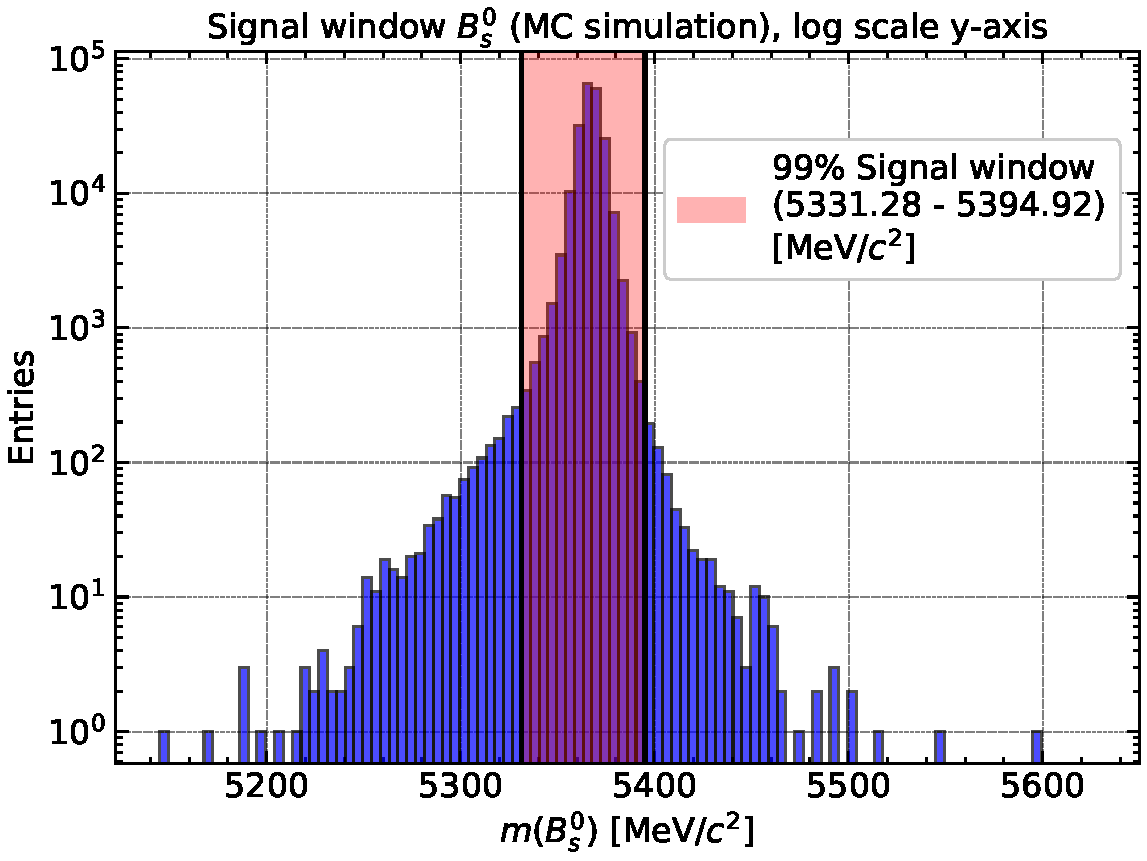
\includegraphics[width=0.3\linewidth]{graphs/sig_window_log.pdf}\label{signalwindow1}}
    \hfill % \hskip 1ex
    \subfloat[Signal window on the LHCb real data.]{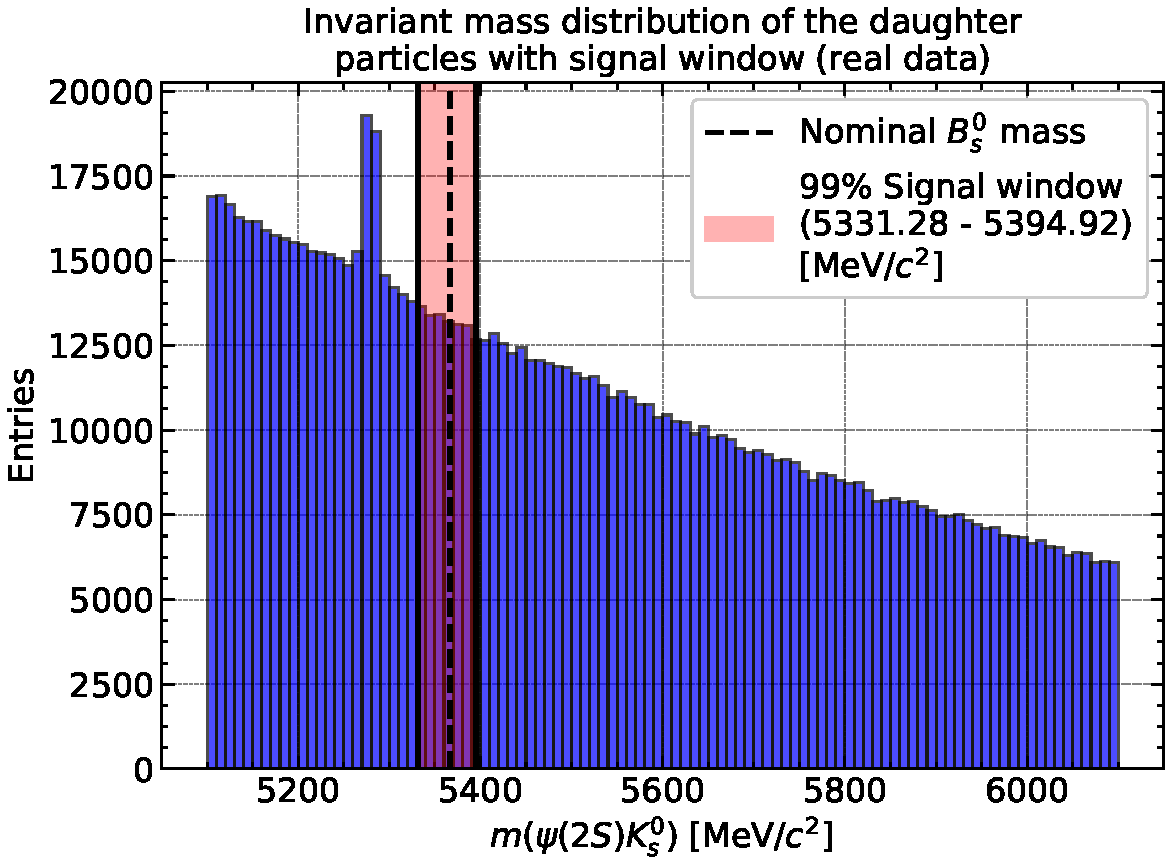
\includegraphics[width=0.3\linewidth]{graphs/sig_window_real.pdf}\label{signalwindow3}}
    \hfill
    \subfloat[Invariant mass distribution of LHCb real data with sWeights.]{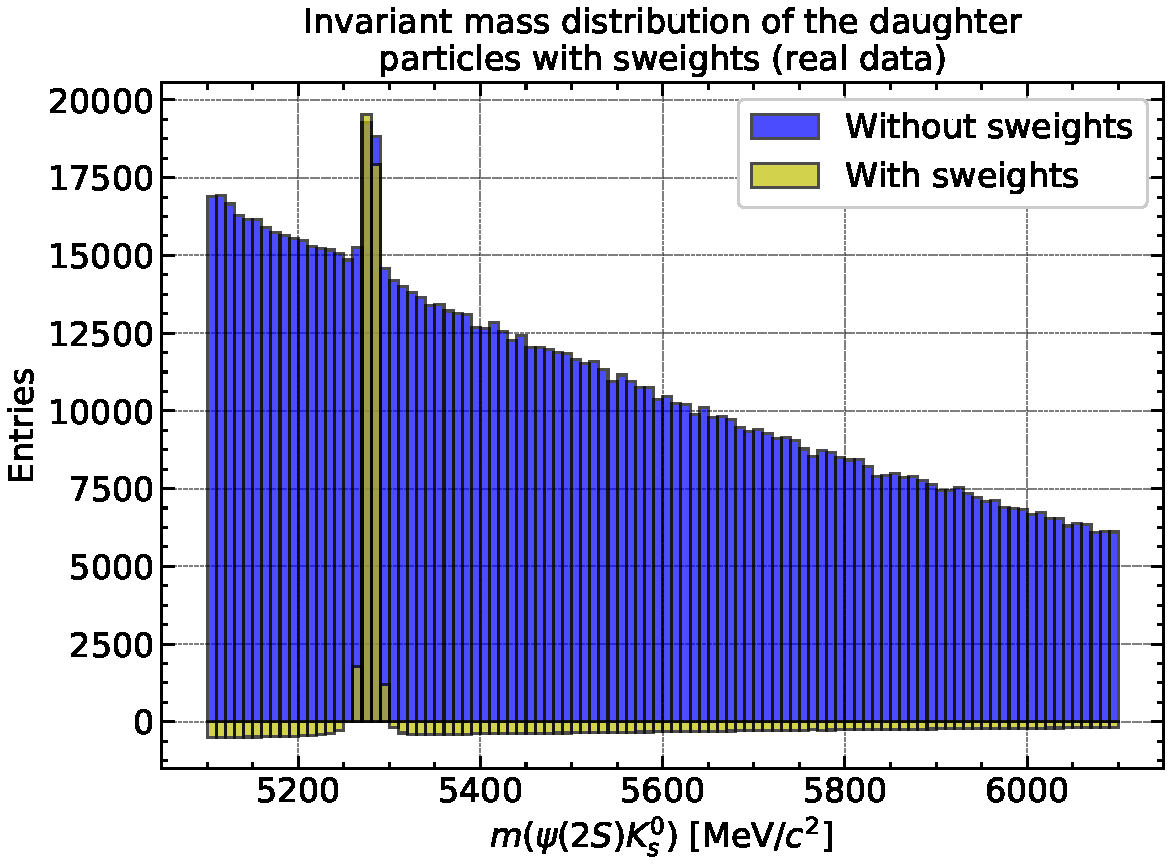
\includegraphics[width=0.3\linewidth]{graphs/sweights.pdf}\label{fig:sub2}}
    \caption{}
\end{figure}

We need to exhibit the problem step by step. First things first, we are going to extract some information from the invariant mass signal distributions for the simulations of $B_s^0$ as well as $B_d^0$ (\Cref{predatasets1} and \Cref{predatasets2}). The mass distribution of $B_s^0$ decay is only a short interval within the LHCb data. In order to isolate it, we define the signal window. We construct an interval centered around the peak with a lower and higher boundary on the invariant mass. We extend the boundaries until 99\% of our simulated $B_s^0$ signal events fall inside as can be seen in \Cref{signalwindow1} (Approximately 3.5 standart deviations of the distribution). As for the $B_d^0$ simulation data, we are going to complement it using sPlot to extract sWeights from the LHCb data and get a fit from real data as can be seen in \Cref{signalwindow3}.\newline

For the background events to be used as non-signal label in the training of the classifier algorithm, we are going to make a cut at the higher limit of the $B_s^0$ simulated signal band and use the upper side band interval where there are no resonances. We will call this interval the \qq{upper side-band background} \Cref{usb}.

\begin{figure}[H]
	\centering
	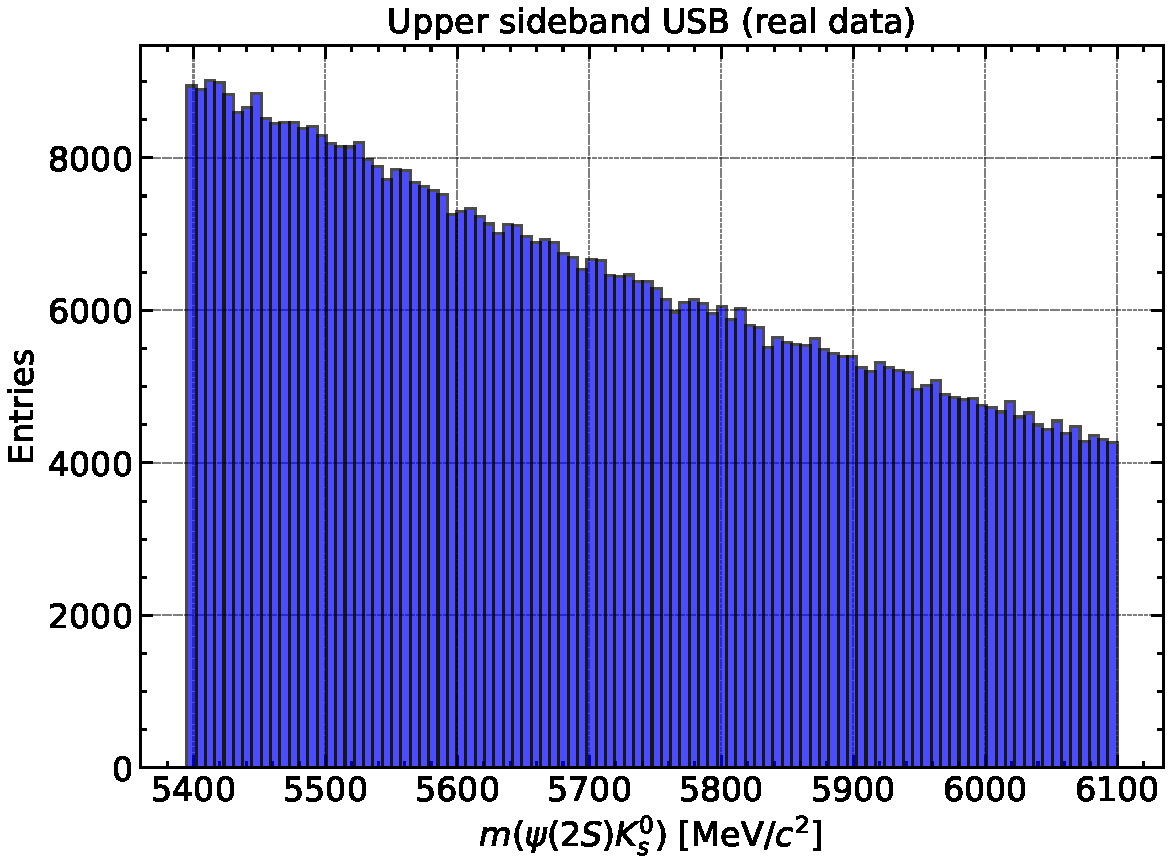
\includegraphics[width=0.6\linewidth]{graphs/USB.pdf}
	\caption{Upper Side-Band Background Region.}
    \label{usb}
\end{figure}

%%------------------------------------------------------%%

\section{Feature Selection}

\begin{figure}[H]
    \centering
    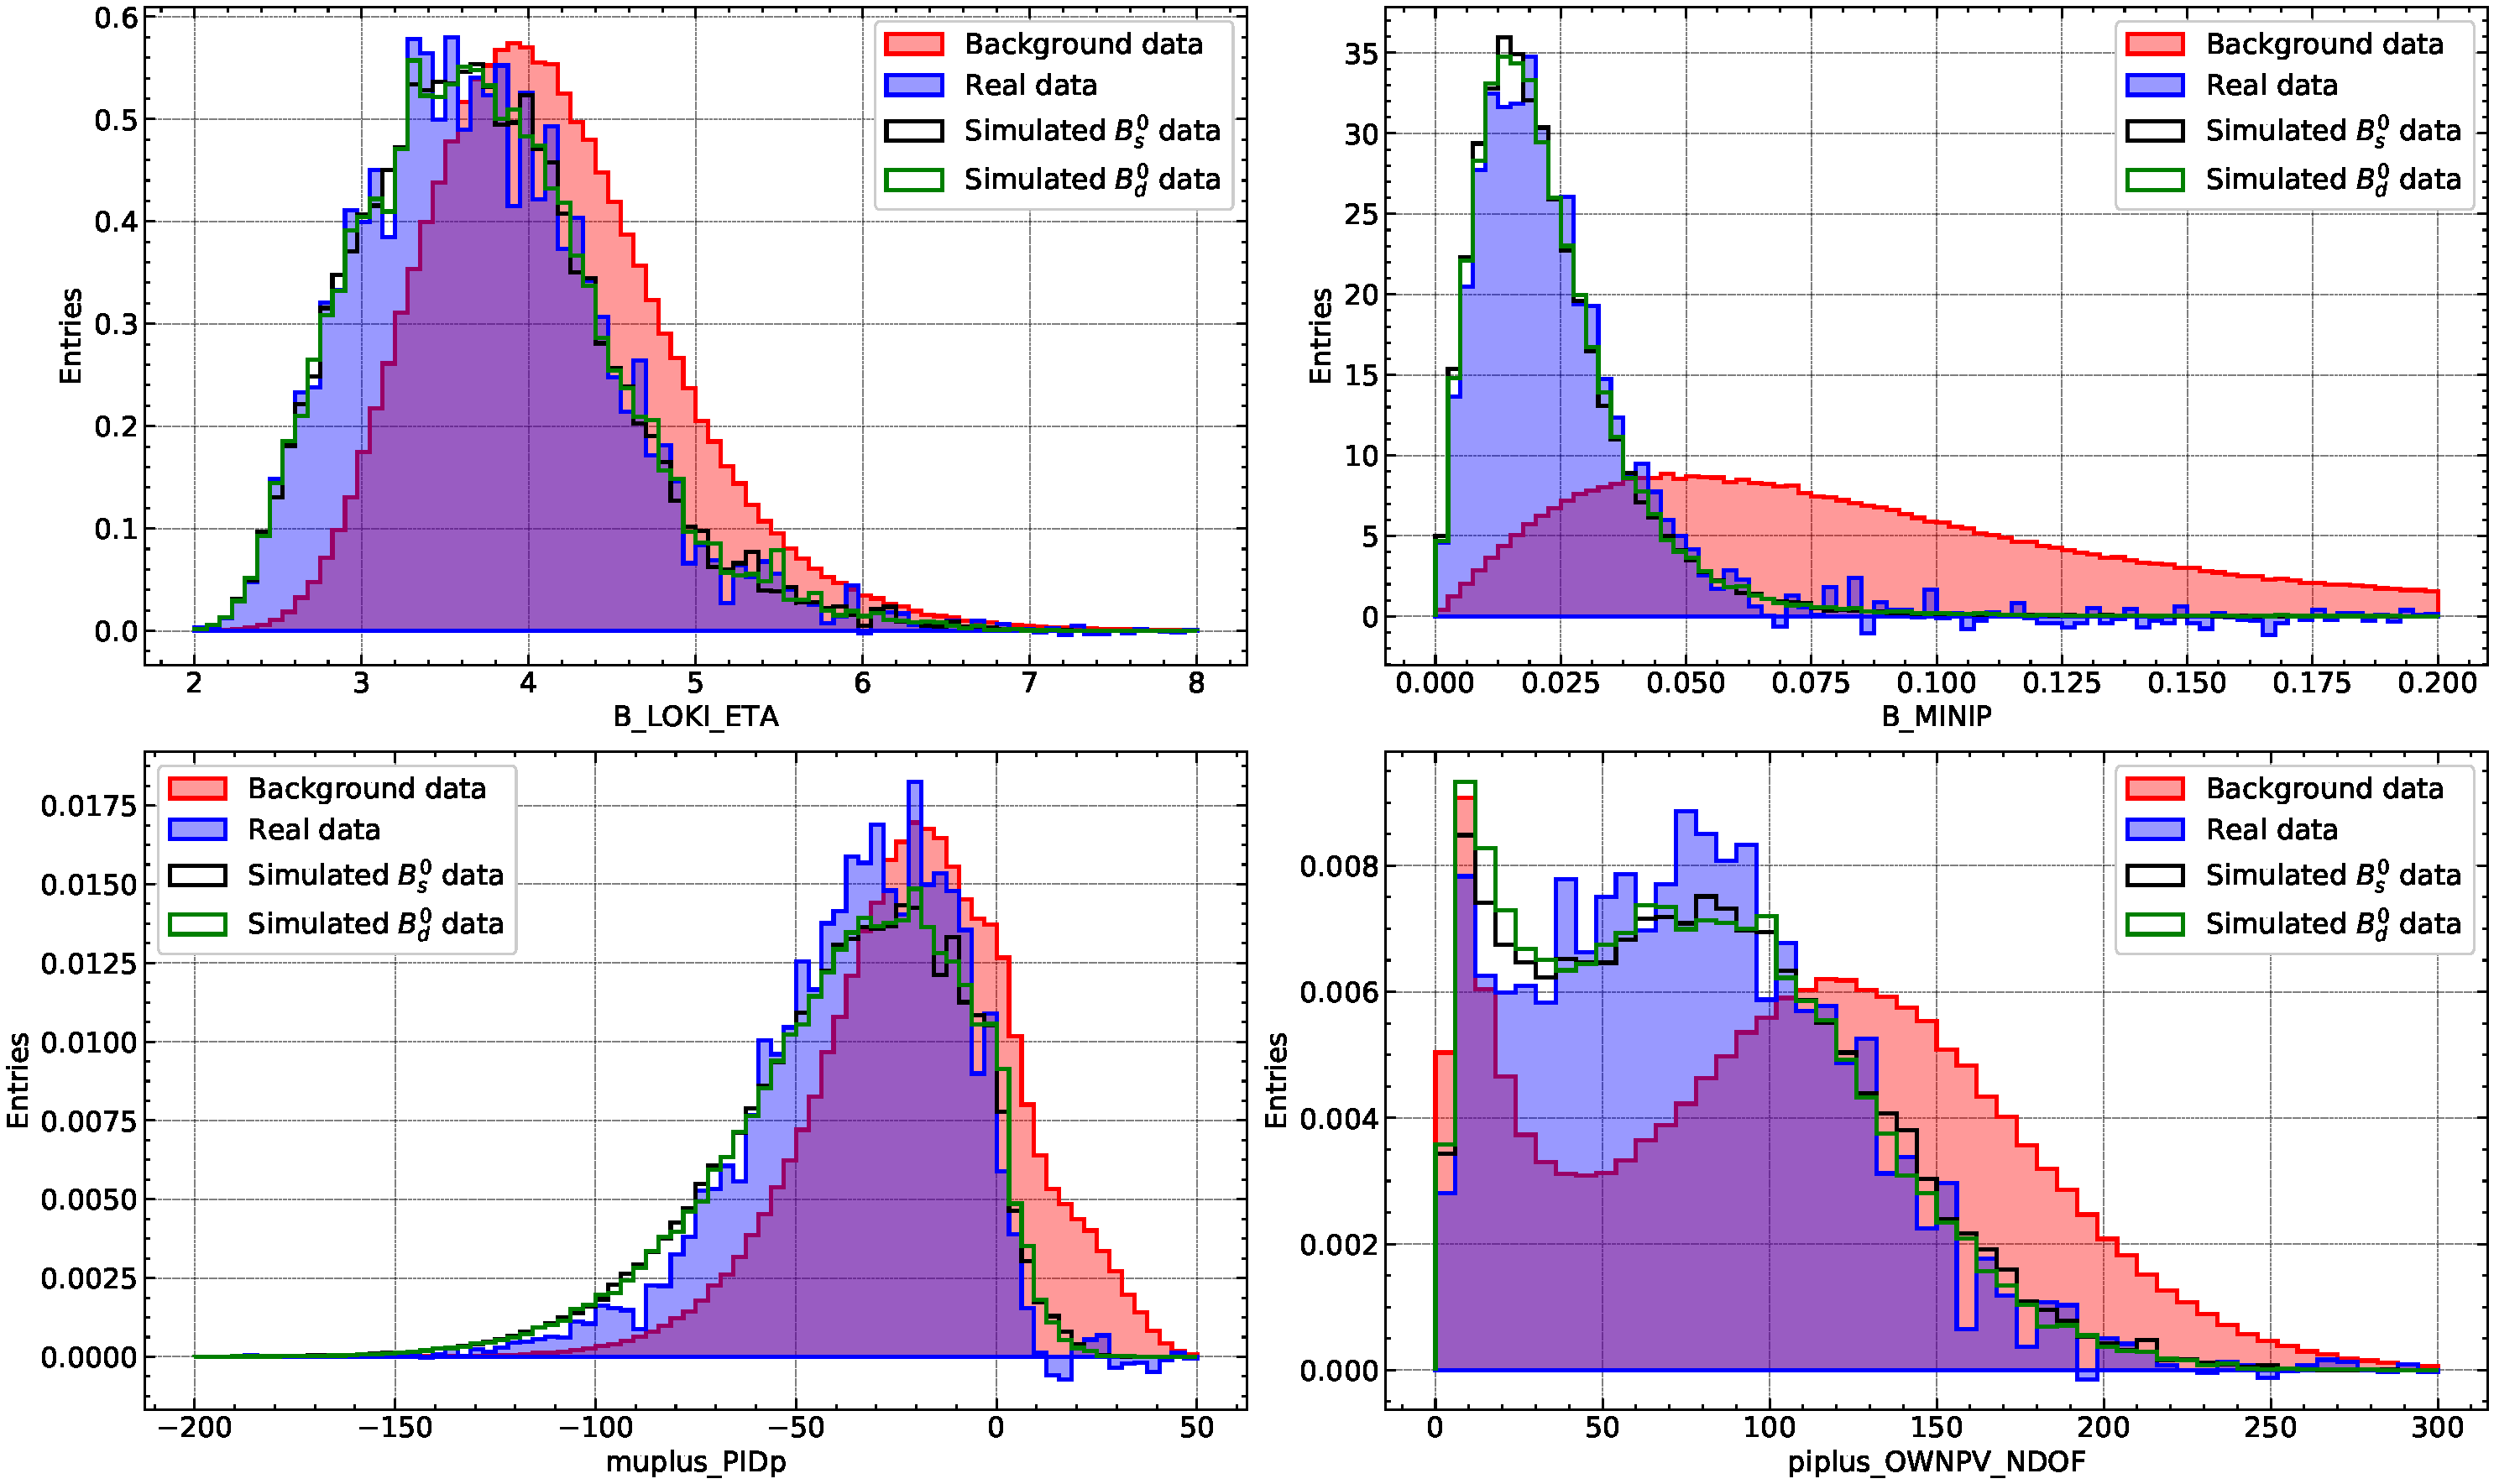
\includegraphics[width=0.8\linewidth]{graphs/features3.pdf}
    \caption{Comparison of 4 feature distributions over the different datasets we have.}
    \label{fig:fea_sel}
\end{figure}

In order to start the training of a multi-variate classifier, we need to pick a number of data \textit{features} out of the 863 that will be used for the training of the machine learning algorithm. First of all, we identify the best features to use in the analysis in three steps.

First step, a selection is made by comparing each feature from the sWeights applied real signal of $B_{d}^{0}$ (blue colour in \Cref{fig:fea_sel}) with the ones from the simulation of $B_{d}^{0}$ (green colour). We utilize the Kolmogorov–Smirnov test to measure the distance between the same features on different datasets and making a cut to keep only the features that fall below a certain distance threshold. Choosing features with minimal distance selects only those with the most similar feature distribution between simulation and real data, so it gives us an idea of how good the simulation is in reproducing the real processes.

The Kolmogorov-Smirnov test \cite{KS_test} keeps the largest distance between the cumulative probability distributions $F^i$:
\begin{equation}
    D_n = \sup_x\left|F_n^1(x)-F_n^2(x)\right|
\end{equation}
where $n$  runs over all bins of the histograms.

Second step, in feature selection, we compare the simulation of $B_{d}^{0}$(green colour) and the background data (red colour) to identify this time the maximal distance between the features and do another selection. In this case we want our model to be able to distinguish and classify signal over background events.

Finally, we have a set of variables that is well simulated and provides good discrimination between signal and background. Last step is to check the correlation of the selected features and discard the ones with an high correlation coefficient in order to avoid biasing our model to the $B_d^0$ simulation.

In Figure \Cref{fig:corr}, we plotted the correlation value for each feature on a colour scale with high colour intensity that corresponds to high correlation.

\newpage
\begin{figure}[H]
    \centering
    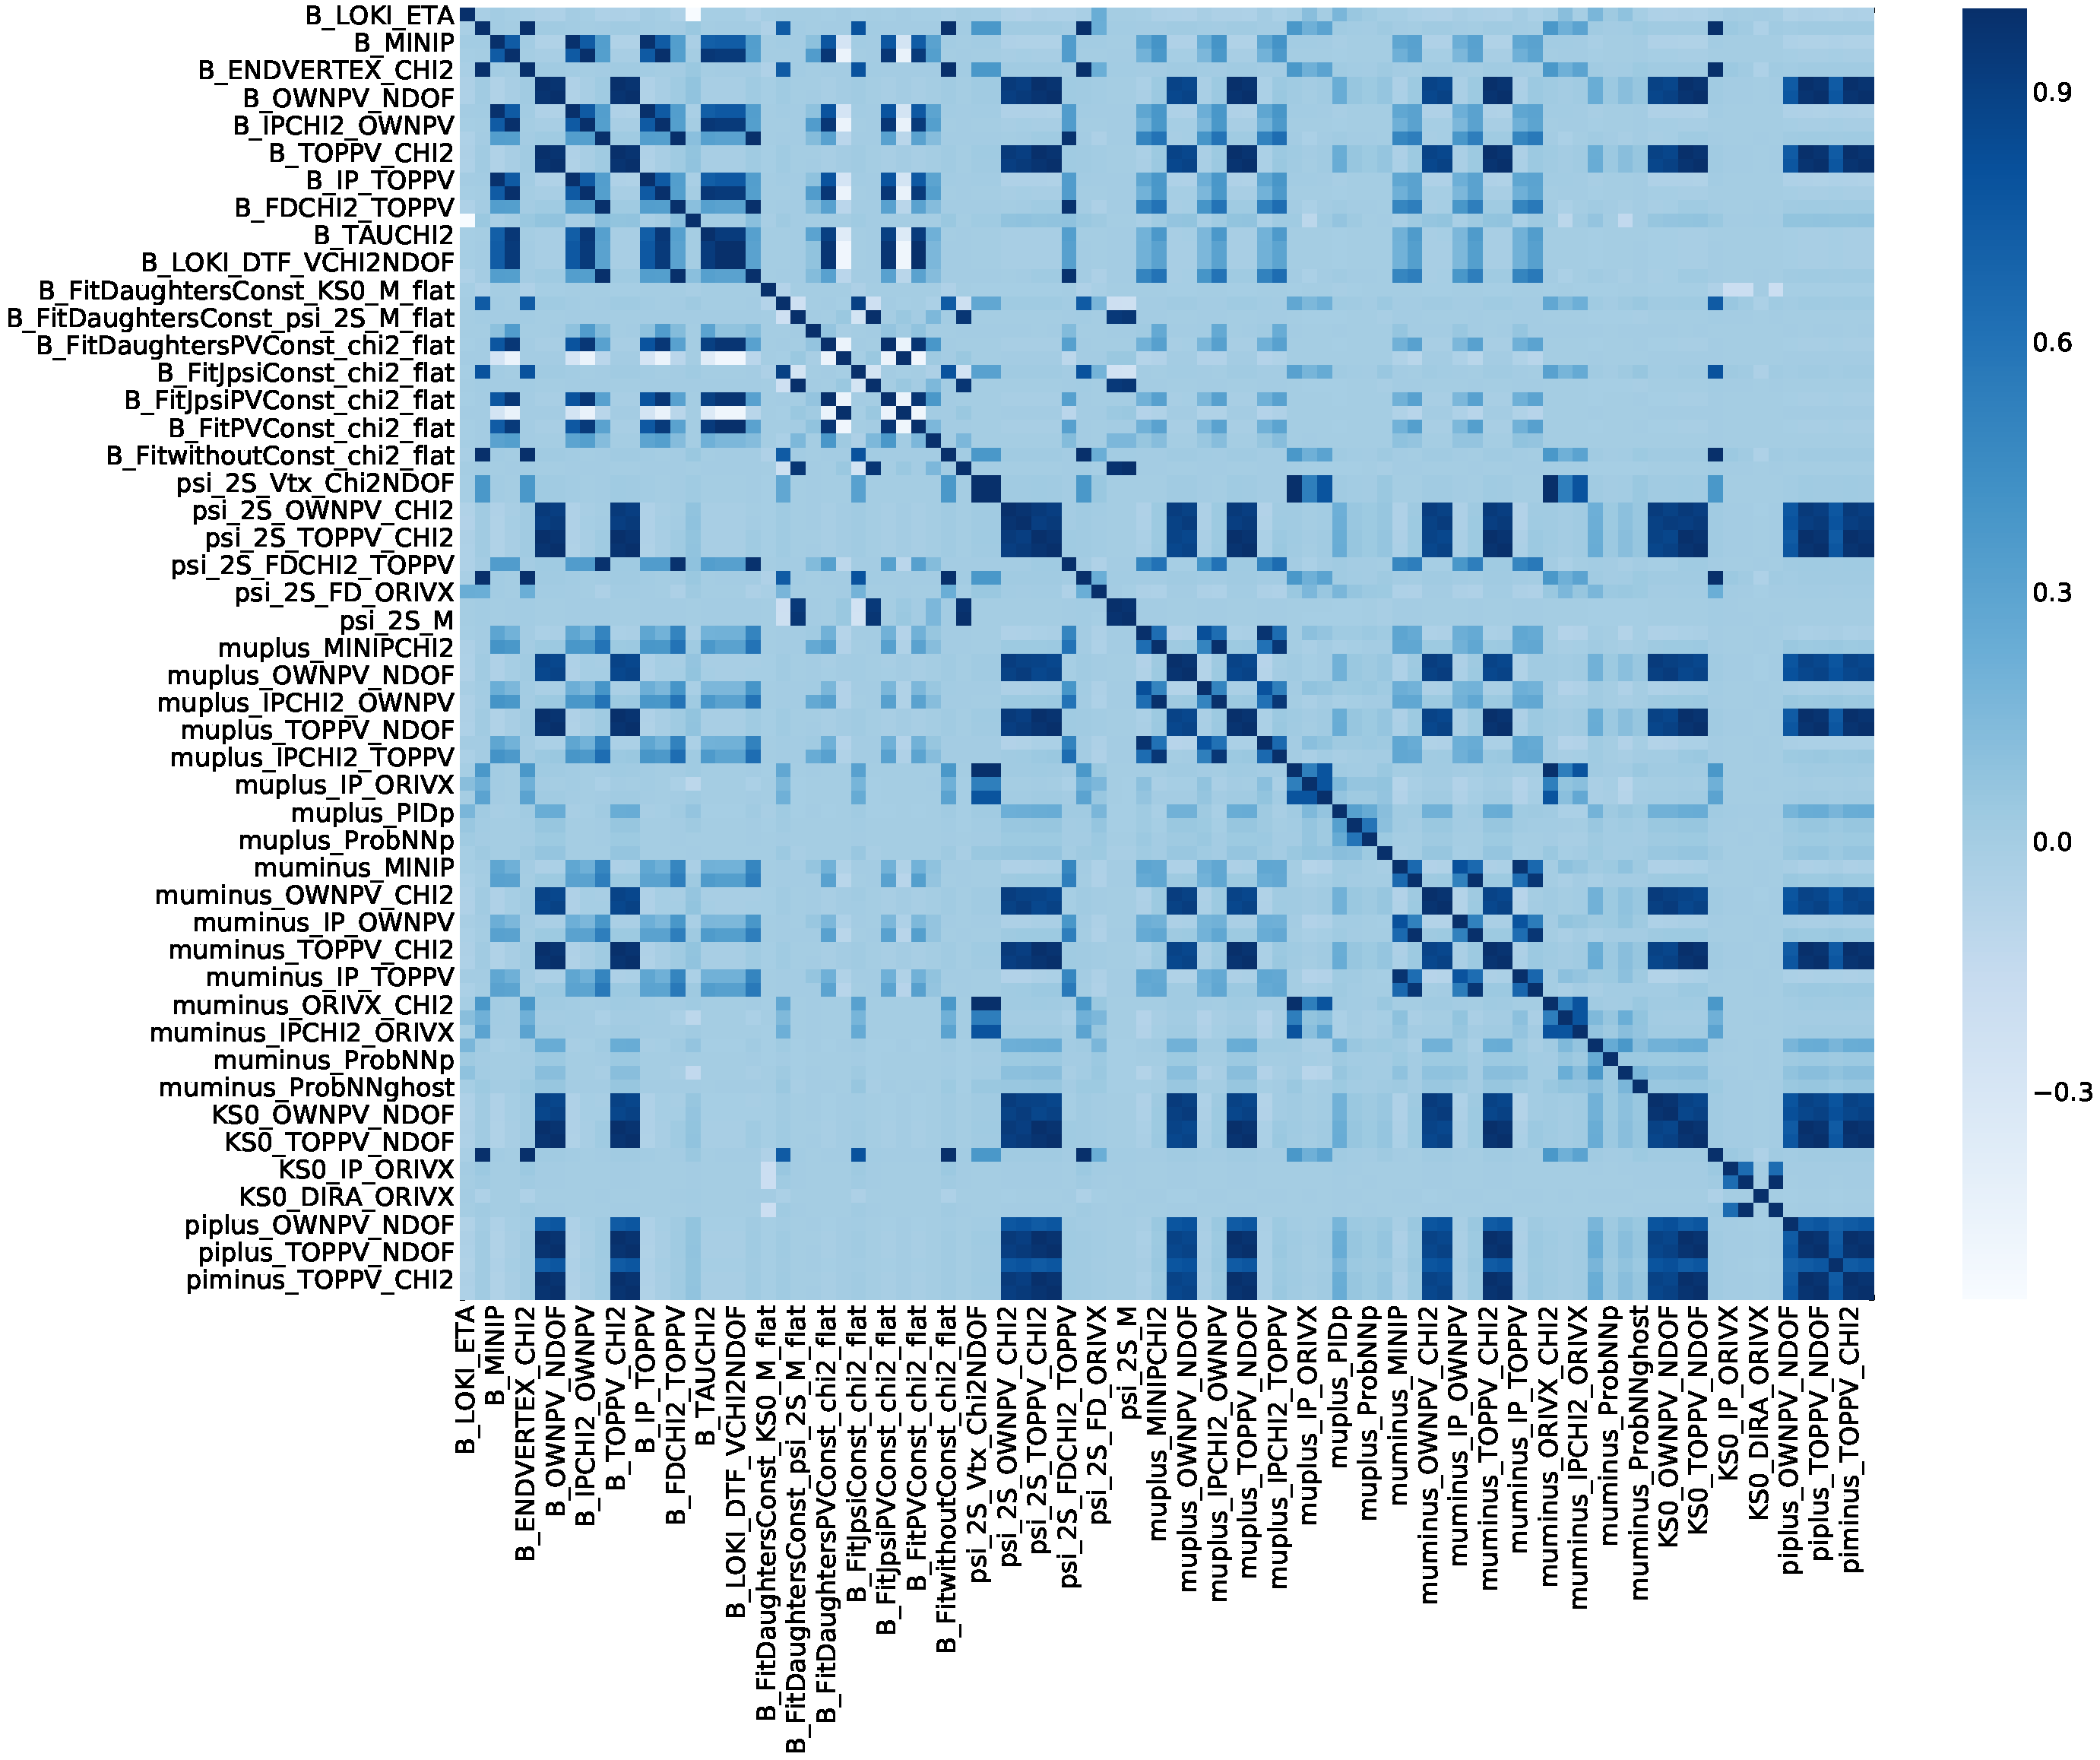
\includegraphics[width=0.95\linewidth]{graphs/corr_big.pdf}
    \caption{Correlation between different features}
    \label{fig:corr}
\end{figure}

%%------------------------------------------------------%%

\section{Model training and multivariate classification}

The multivariate classifier learner we chose to use for this analysis is a gradient boosted decision tree in the $\texttt{XGBoost}$ package \cite{Chen}. A Boosted Decision Tree (BDT) is a powerful machine learning method that builds an ensemble of decision trees in a sequential manner, where each new tree is trained to correct the errors made by the previous ones. The $\texttt{XGBoost}$ (Extreme Gradient Boosting) package is a widely-used implementation of gradient-boosted decision trees, especially in classification tasks.

Since the background training dataset is much larger than the signal training dataset, the background data will be weighted so that the classifier can be trained equally on signal and background samples:
\[
\text{weight}=\frac{\text{\textbf{\#}signal}}{\text{\textbf{\#}background}}
\]

\begin{center}
\begin{tabular}{||c c c||} 
 \hline
 \textbf{\#}signal & \textbf{\#}background & weight \\ [0.5ex] 
 \hline
 211314 & 643816 & 0.3282 \\ 
 \hline
\end{tabular}
\end{center}

\subsection{Boosted Decision Tree}

For the classification, we train five BDTs on a 5-fold cross validation: this procedure consists of splitting the data into $k$ subsamples and use $k-1$ of those for the training ad the other one for the testing; and then repeating for $k$ times. Cross validation is used to avoid \emph{overfitting}, indeed no one specific subsample is used for final validation of the classifier.

To measure the performance of a BDT we look at quantities like the true positive rate (TPR) and the false positive rate (FPR), meaning those events that the model has failed to classify correctly in the testing procedure. Our aim is to train the model to be as precise as possible and so, to minimize this the FPR while keeping the TPR high.

\begin{figure}[H]
    \centering
    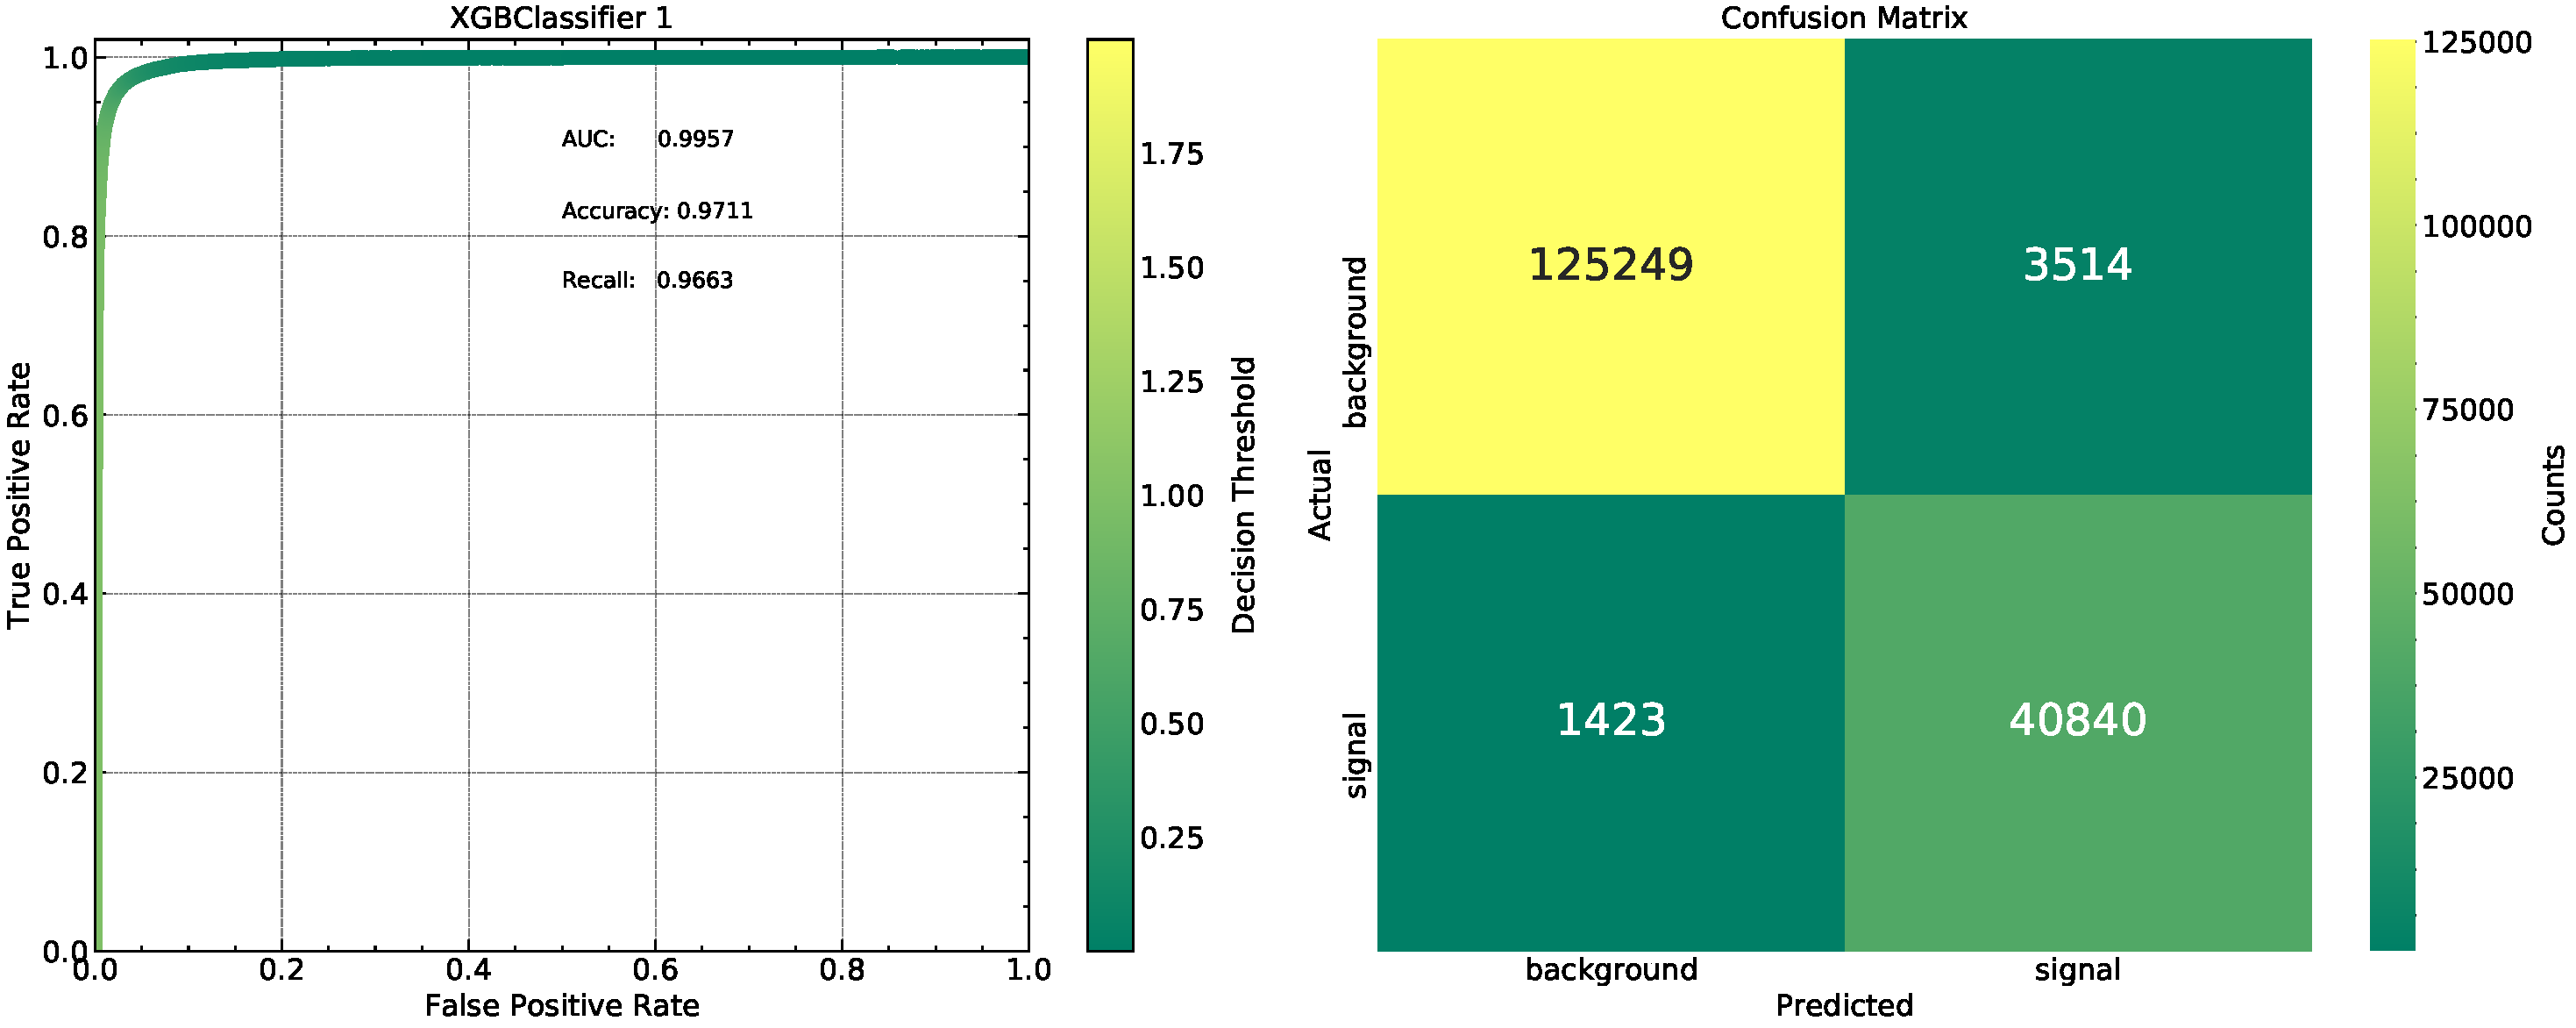
\includegraphics[width=0.90\linewidth]{graphs/clf0.pdf}
    \caption{ROC curve of the first trained XBG Classifier (\emph{left}); Confusion matrix of the first trained XBG Classifier (\emph{right}).}
    \label{roc}
\end{figure}

When plotted together to a normalized value of $1$, the TPR and FPR make up the "Receiver Operator Characteristics (ROC)" curve and the area under the curve (AUC) ranks the accuracy of the learner from $0$ to $1$; $1$ being a perfect score \cite{roc}. An example of the ROC results from the first of $5$ BDT's is shown in \Cref{roc}.

\begin{figure}[H]
    \centering
    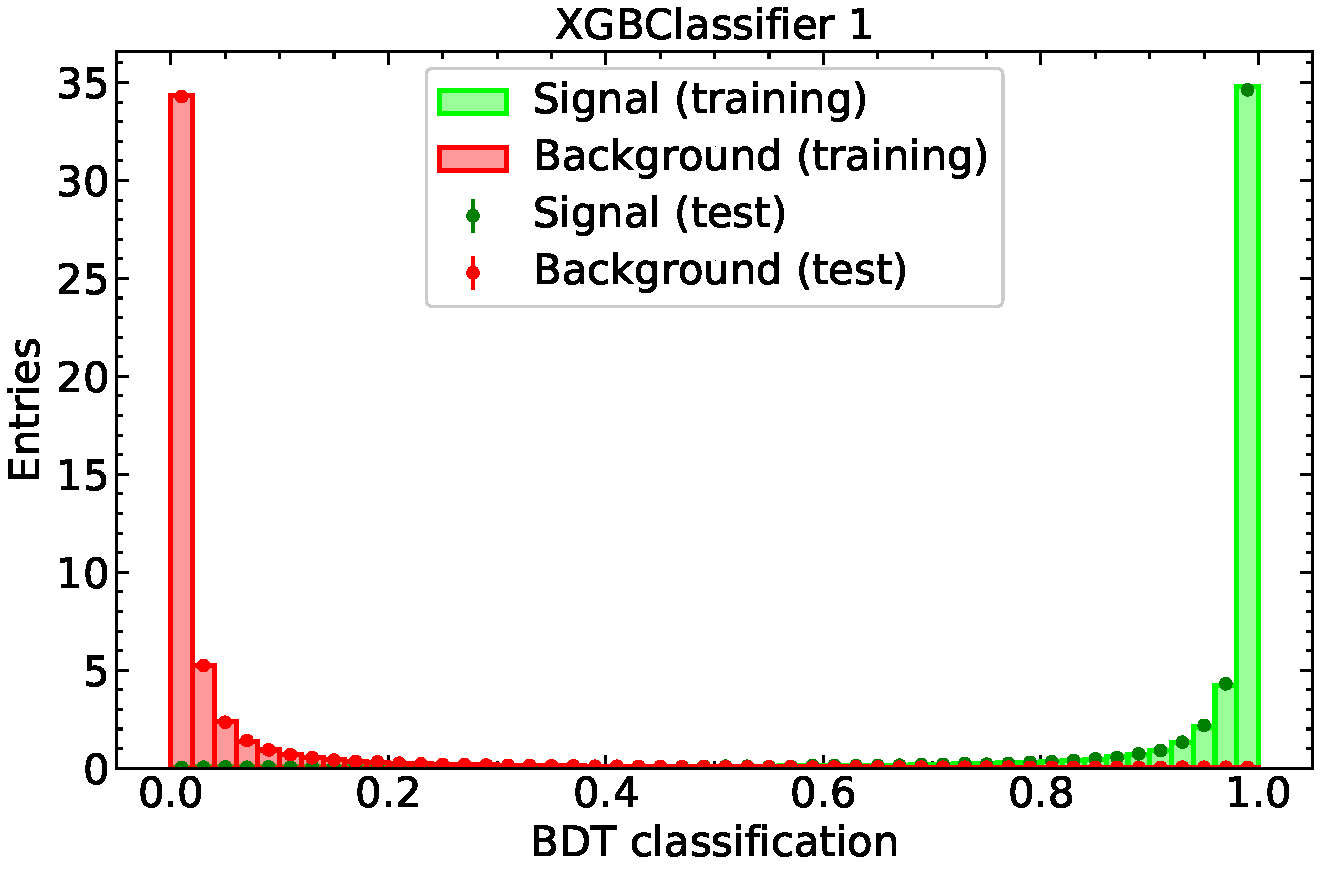
\includegraphics[width=0.6\linewidth]{graphs/train_test0.pdf}
    \caption{Accuracy test of the first iteration of BDT classifier.}
    \label{traintest}
\end{figure}

To check for overtraining, the output of the first classifier is histogramed on training and test data \Cref{traintest}. The agreement of the histograms columns and the points is a good sign that no overtraining has occurred.

\subsection{Classification threshold}
Once we complete the training and testing procedure with the 5-fold cross validation, we have to find out a suitable \emph{threshold} value (between 0 and 1).

We use the Punzi figure of merit (FOM), \Cref{eq:punzi}: for varying threshold values, the signal efficiency and number of
background events in the signal window is computed. In particular, the number of background events in the signal window is computed by
fitting an exponential background model to the upper sideband and extrapolating the number of events in the desired signal region. We repeat this for all five BDTs and then we compute the best threshold cut, taking the average of the threshold of each BDT.

An entry beyond this best threshold will be considered as a signal in our classifier.

\begin{figure}[H]
    \centering
    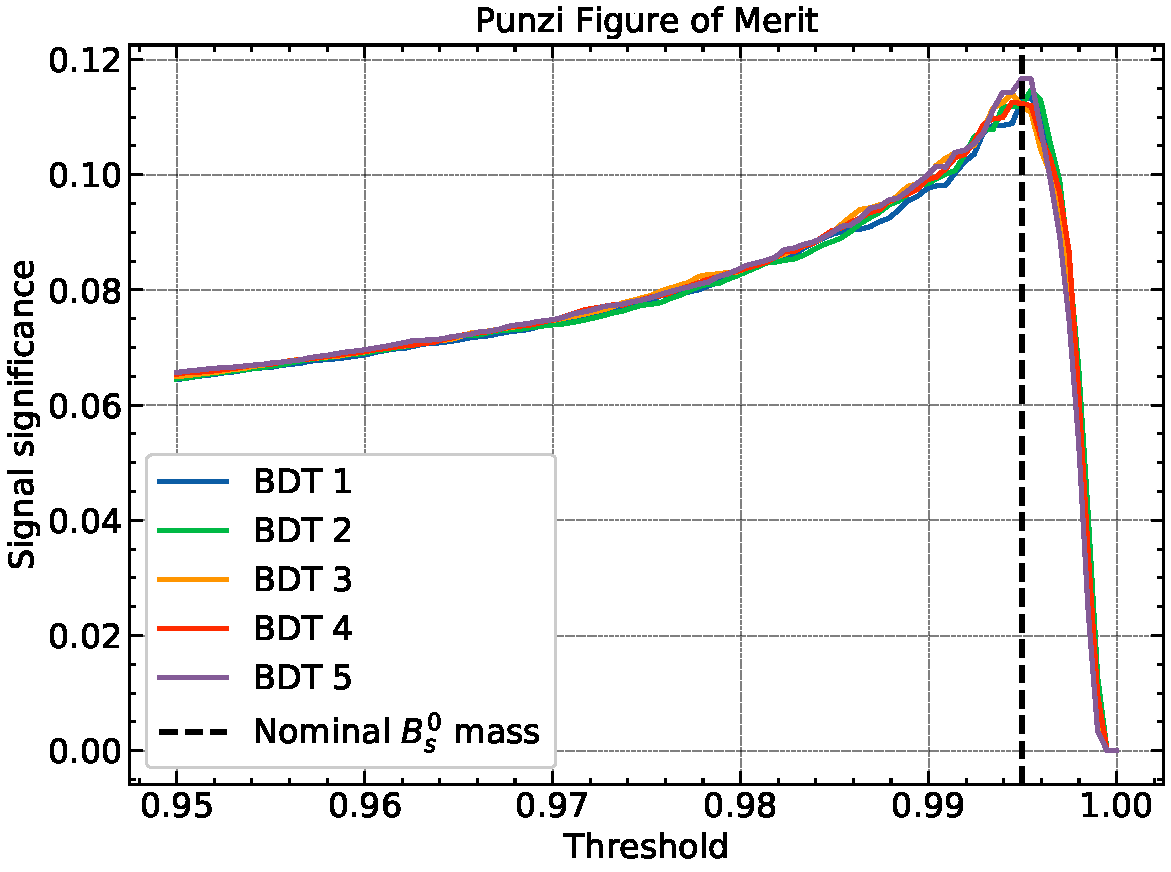
\includegraphics[width=0.6\linewidth]{graphs/punzi.pdf}
    \caption{Punzi FOM results for all 5-fold BDT.}
    \label{punzi}
\end{figure}

For our classifier, the best threshold happens to be 0.995 (\Cref{punzi}).

%%------------------------------------------------------%%

\section{Invariant mass fit}
We apply the best threshold cut to the data predicted by the BDT models, obtaining the distribution plotted in \Cref{BDT}:

\begin{figure}[H]
    \centering
    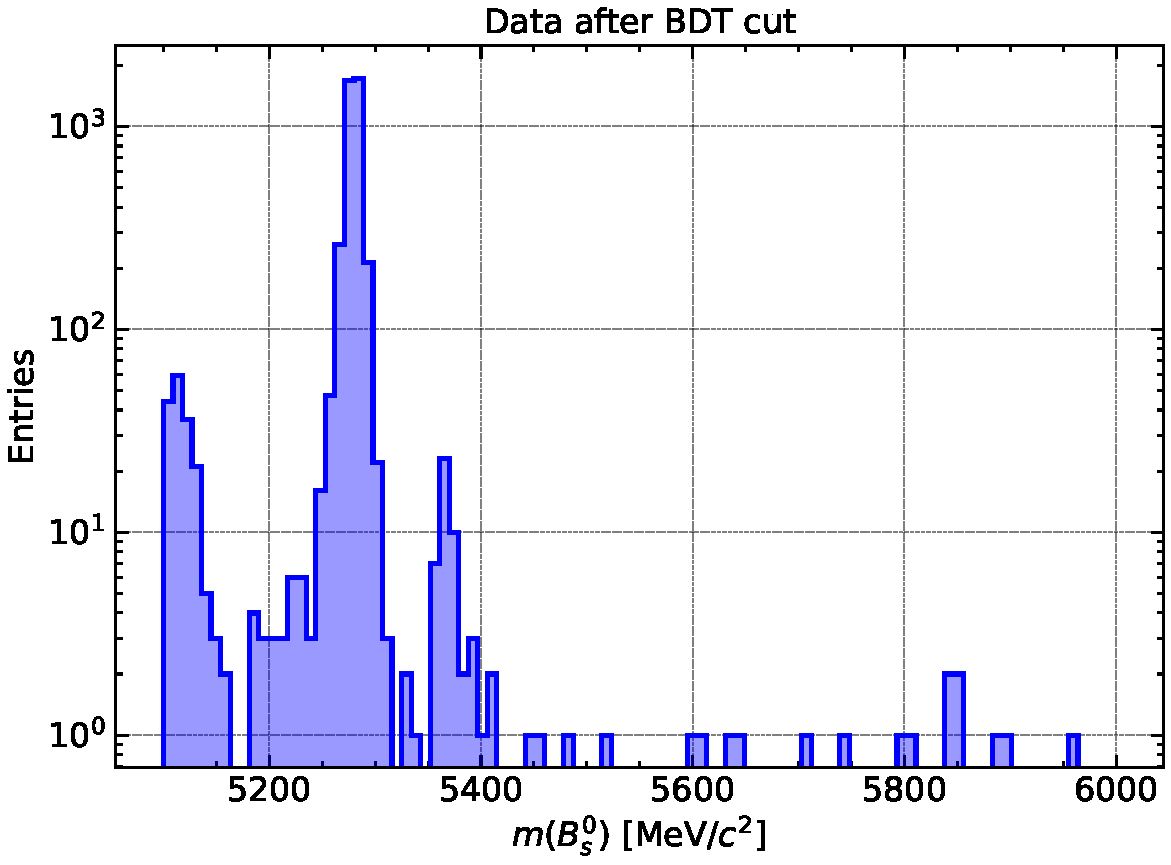
\includegraphics[width=0.70\linewidth]{graphs/dataBDTcut.pdf}
    \caption{BDT real data invariant mass distribution after the threshold cut.}
    \label{BDT}
\end{figure}

Here we have to notice that in the distribution, obtained from the classifier, we can (still) identify the $B_d^0$ peak and now the $B_s^0$ peak too.

Now, we have to find out what signal and background yield we are getting here. Therefore, we need to model the entire distribution: our model consist of two Gaussians (for each of the two mass peaks) and one exponential background component.
The two Gaussian peaks are defined as:

\begin{equation}
    G(m) = \frac{r}{\sqrt{2 \pi} \sigma_1} \exp \left[-\frac{\left(m-\mu_1\right)^2}{2 \sigma_1^2}\right]+ \frac{(1-r)}{\sqrt{2 \pi} \sigma_2} \exp \left[-\frac{\left(m-\mu_2\right)^2}{2 \sigma_2^2}\right]
\end{equation}

where $\mu_i$ and $\sigma_i$ are the mean and width of the two Gaussians, $r$ is the ratio of the two distributions in the model.

So the full-fit model is defined as

\begin{equation}
    F_{\text{full}}(m) = \alpha \cdot G_{B_s^0}(m) + \beta \cdot G_{B_d^0}(m) + \gamma \cdot e^{- \delta \cdot m}
\end{equation}

where $G_{B_s^0}(m)$ and $G_{B_d^0}(m)$ are the Gaussian model used to fit the two $B_s^0$ and $B_d^0$ distributions and $\alpha$, $\beta$, $\gamma$, $\delta$ are free parameter of the model, to be determined.

In order to build a stable model, we firstly (pre-)fit the peaks to their respective simulation distribution so that we fix the mean and width of both signal samples, respectively. (To ensure that the peaks in the simulation match the peak shape in the data, we have classified both signal samples and applied the BDT cut \underline{before} performing the fit).

After that, the only free parameters of the final fit are the background yield, the $B_s^0$ and $B_d^0$ signal yield, and the slope of the exponential combinatorial background. The plot of the full-fit is in \Cref{fit}:

\newpage
\begin{figure}[H]
    \centering
    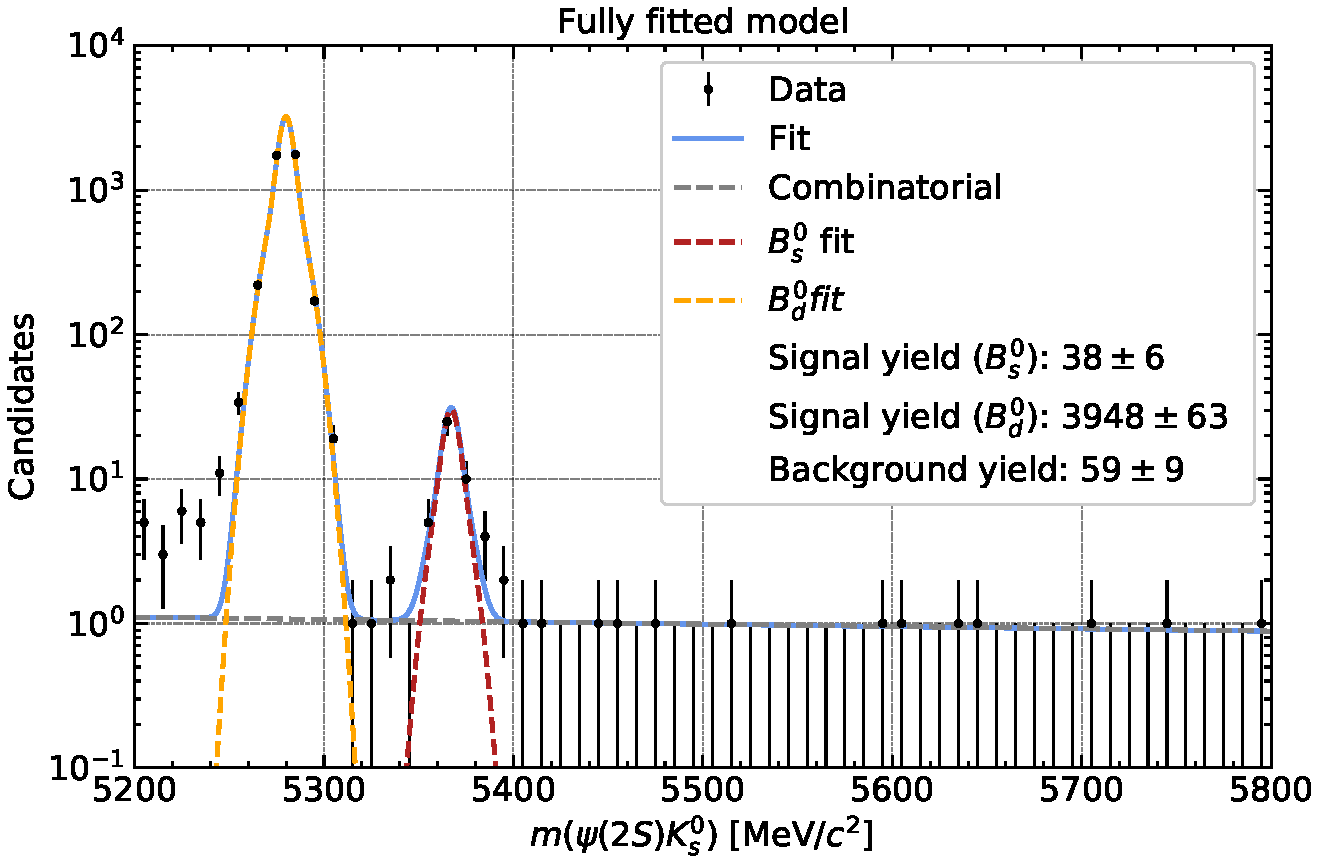
\includegraphics[width=0.70\linewidth]{graphs/plot_fit.pdf}
    \caption{Fit of the BDT classified data on the invariant mass range for reconstructed final products of $B_{s}^{0}$ decay.}
    \label{fit}
\end{figure}

Finally, with the parameters obtained from the fit, we can obtain the number of signal and background event, needed to compute \Cref{eq:sig}, integrating over the $B_s^0$ peak and the exponential background.

The obtained significance is:
\begin{equation}
    m=5.68 \hspace{0.1em} \sigma
\end{equation}
%%------------------------------------------------------%%
